\documentclass[12pt, a4paper]{article}
\usepackage[top=1.0in, bottom=1.0in, left = .8in, right=.8in]{geometry}
\usepackage{graphicx}
\usepackage{amsmath}
\usepackage{listings}
\usepackage{xcolor}
\usepackage{amssymb}
\usepackage{paracol}
\usepackage{physics}

\newcommand{\appropto}{\mathrel{\vcenter{
  \offinterlineskip\halign{\hfill $##$\cr
    \propto\cr\noalign{\kern2pt}\sim\cr\noalign{\kern-2pt}}}}}
\usepackage{mathtools}

\usepackage[utf8]{inputenc}

\usepackage{listings}
\usepackage{xcolor}

\definecolor{codegreen}{rgb}{0,0.6,0}
\definecolor{codegray}{rgb}{0.5,0.5,0.5}
\definecolor{codepurple}{rgb}{0.58,0,0.82}
\definecolor{backcolour}{rgb}{0.95,0.95,0.92}

\lstdefinestyle{mystyle}{
    backgroundcolor=\color{backcolour},   
    commentstyle=\color{codegreen},
    keywordstyle=\color{magenta},
    numberstyle=\tiny\color{codegray},
    stringstyle=\color{codepurple},
    basicstyle=\ttfamily\footnotesize,
    breakatwhitespace=false,         
    breaklines=true,                 
    captionpos=b,                    
    keepspaces=true,                 
    numbers=left,                    
    numbersep=5pt,                  
    showspaces=false,                
    showstringspaces=false,
    showtabs=false,                  
    tabsize=2
}

\lstset{style=mystyle}

\title{\textbf{Assignment 9 : The Digital Fourier Transform}} % Title
\author{\textbf{Gagan Deep Goru}} % Author name
\date{\today} % Date for the report
\begin{document}		
\maketitle % Insert the title, author and date
\section*{Introduction} 
In this assignment, we explore the way of computing Discrete Fourier Transform and try to recover the analog fourier transform by proper sampling of the signal.
\section{Given Examples}
This section is all about working through the given examples in the document. We first start with the DFT of $\sin(5t)$. The fourier transfrom of this function is:
\begin{equation*}
Y(\omega) = \frac{1}{2j}[\delta(\omega - 5) - \delta(\omega + 5)]
\end{equation*}
We see that the fourier transform has two impulses one at 5 and the other at -5, each with strength of 0.5. The discrete fourier transform is computed using the following code, and it is plotted. The plot is shown in Figure 1. In the phase plot, only the points where the frequencies had significant strength are plotted.\\

\lstset{language=Python}
\lstset{frame = lines}
\lstset{label={lst:code_direct}}
\lstset{basicstyle=\footnotesize}
\begin{lstlisting}	
t = np.linspace(0, 2*np.pi, 129)
t = t[0:-1]
y = np.sin(5*t)
Y = np.fft.fftshift(np.fft.fft(y))/128.0
\end{lstlisting}

\begin{figure}
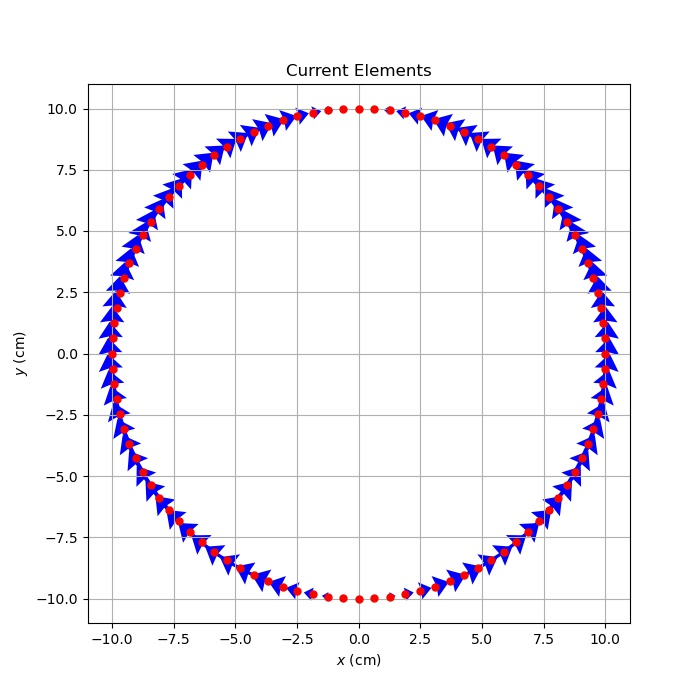
\includegraphics[scale=1]{fig1.jpeg}
\caption{Spectrum of $\sin(5t)$}
\end{figure}

\begin{flushleft}
The second example is $(1 + 0.1\cos(t))\cos(10t)$. The fourier transform of this function is computed as:
\begin{equation*}
y(t) = \cos(10t) + 0.1\cos(t)\cos(10t)
\end{equation*}
\begin{equation*}
\Rightarrow y(t) = \cos(10t) + 0.05\cos(9t) + 0.05\cos(11t)
\end{equation*}
\begin{equation*}
\Rightarrow Y(\omega) = \frac{1}{2}[\delta(\omega - 10) + \delta(\omega + 10) + 0.05\delta(\omega - 9) + 0.05\delta(\omega + 9) + 0.05\delta(\omega - 11) + 0.05\delta(\omega + 11)]
\end{equation*}
We can see that there are 6 impulses, at 9, 10, 11 and at -9, -10, -11. The impulses are 9, 11, -9, -11 have relatively less strength than the ones at 10, -10. The plot is shown in Figure 2.
\end{flushleft}
\begin{figure}
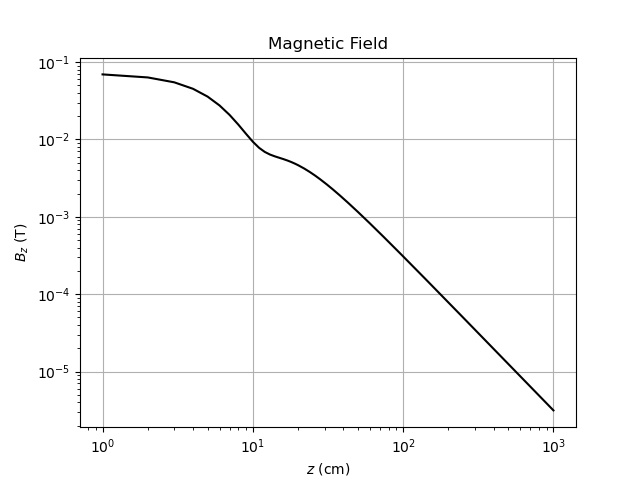
\includegraphics[scale=1]{fig2.jpeg}
\caption{Spectrum of $(1 + 0.1\cos(t))\cos(10t)$}
\end{figure}

\section{Spectrum of Cubed Sinusoids}
In this section we compute and plot the spectra of $\sin^3(t)$ and $\cos^3(t)$. The frequency components in these functions can be seen as:
\begin{equation*}
\sin^3(t) = \frac{3\sin(t) - \sin(3t)}{4}
\end{equation*}
\begin{equation*}
\cos^3(t) = \frac{3\cos(t) + \cos(3t)}{4}
\end{equation*}
We see that both functions have frequencies of 1 and 3. This can be seen from the plots of their Spectra. The plots are shown in Figures 3 and 4.

\begin{figure}
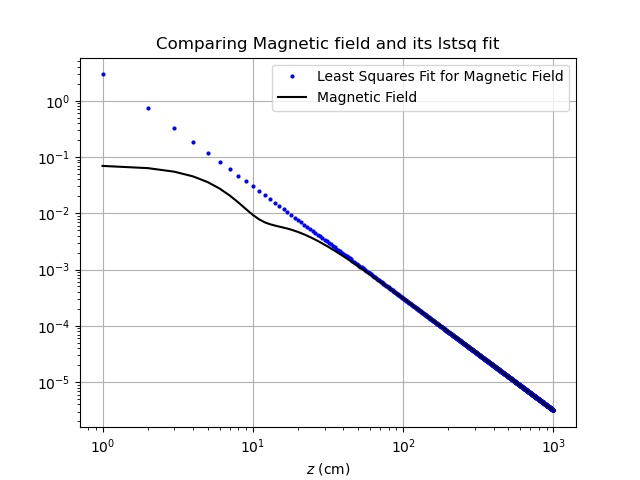
\includegraphics[scale=1]{fig3.jpeg}
\caption{Spectrum of $\sin^3(t)$}
\end{figure}

\begin{figure}
\includegraphics[scale=1]{fig4.jpeg}
\caption{Spectrum of $\cos^3(t)$}
\end{figure}

\section{DFT of a Frequency Modulated Signal}
In this section, we calculate the spectrum of the frequency modulated signal $\cos(20t + 5\cos(t))$. The frequency of this signal varies from 15 to 25 continuously. So, instead of a single spike, we see many spikes between 15 and 25. The plot is shown in figure 5.

\begin{figure}
\centering
\includegraphics[scale=1]{fig5.jpeg}
\caption{Spectrum of $\cos(20t + 5\cos(t))$}
\end{figure}

\section{DFT of Gaussian}
The Gaussian is not a periodic signal. But in order to get DFT, we need samples of a periodic signal, otherwise the frequency information can't be fit into a finite number of samples. Hence, we consider a new signal, which is same as the Gaussian for a window $[\frac{-T}{2}, \frac{T}{2}]$. Since the Gaussian becomes very small away from the origin, we can find a sufficiently big window for the required accuracy. We can write the Fourier Transform as:
\begin{align*}
X(\omega) &= \int_{-\infty}^{\infty} x(t)e^{-j\omega t} dt \\
\Rightarrow X(\omega) &\approx \int_{-T/2}^{T/2} x(t)e^{-j\omega t} dt \\
\Rightarrow X(\omega) &\approx \sum\limits_{n = \frac{-N}{2}}^{\frac{N}{2}} x(n\Delta t)e^{-j\omega n\Delta t} \Delta t \\
\Rightarrow X(\omega) &\approx \Delta t\ DFT\{x(n\Delta t)\}
\end{align*}
Here, $\Delta t$ is $\frac{T}{N}$. The following code is used to find the window T and number of samples N which gives the required accuracy.
\begin{lstlisting}
T = 2*np.pi
N = 128
tol = 1e-6
err = 1

while True:
    t = np.linspace(-T/2, T/2, N+1)[:-1]
    y = np.exp(-t**2/2)
    y = np.fft.fftshift(y)
    Y = np.fft.fftshift(np.fft.fft(y))*T/N
    w = np.linspace(-N*np.pi/T, N*np.pi/T, N+1)[:-1]
    Yw = np.sqrt(2*np.pi)*np.exp(-w**2/2)
    err = np.absolute(Y - Yw).max()
    if err < tol:
        print(f'The error is {err}')
        print(f'Time window is [{-T/2}, {T/2}]')
        print(f'Number of samples N = {N}')
        break
    T *= 2
    N *= 2
\end{lstlisting}
The output for this code is given below, and the plots of the estimated spectrum and true spectrum of the Gaussian are given in Figures 6 and 7.
\begin{verbatim}
The error is 8.382019522912287e-10
Time window is [-6.283185307179586, 6.283185307179586]
Number of samples N = 256
\end{verbatim}

\begin{figure}
\centering
\includegraphics[scale=1]{fig6.jpeg}
\caption{Estimated Spectrum of the Gaussian}
\end{figure}

\begin{figure}
\centering
\includegraphics[scale=1]{fig7.jpeg}
\caption{True Spectrum of the Gaussian}
\end{figure}

\section*{Conclusion}
We used the fft algorithm available in numpy to compute the DFT of various signals and recovered the analog fourier transform from them. We also saw how the fourier transform of non-periodic signals can be generated using DFT.
\end{document}
